\section{Programos sudarymas ir rezultatai}

Pagal dviejų dimensijų skaitinį modelį \eqref{numerical-eqs} sudarytas uždavinį sprendžiantis skriptas ir kiti pagalbiniai skriptai duomenims vaizduoti ir tikrinti. Skriptai rašomi \textit{Python} programavimo kalba, naudojant \textit{NumPy}, \textit{SciPy}, \textit{Matplotlib} paketus. 

Modelio rezultatai yra saugomi kaip atskiri \textit{.npy} formato failai, kurie yra skirti saugoti \mbox{\textit{NumPy}} masyvus. Dėl praktinių rezultatų panaudojimo ir tyrimo nebūtina saugoti informacijos apie visus laiko žingsnius, todėl išsaugotuose rezultatų failuose, simuliacijos kadrai laiko kryptimi gali būti praretinti iki tūkstančio kartų, priklausomai nuo pasirinktų parametrų. Pagalbiniai duomenų vaizdavimo skriptai šiuos duomenis agreguoja į grafikus, kurie išsaugomi \textit{.png} formatu.

\subsection*{Medžiagos kiekis}

Dėl didelės rezultatų dimensijos būtų sunku interpretuoti grafiškai pavaizduotus sprendinio duomenis, todėl tyrimui yra naudinga vizualizuoti ir medžiagų kiekius sistemoje. Galime išskleisti formulę medžiagos kiekiui bendru atveju \eqref{quantity-general} ir gausime formulę diskrečiam atvejui \cite{strangCalculusVolume32016}:
\begin{align}
    q(t) = \int_\Omega c\,dV = \int_0^W \int_0^H c(x, y, t)\,dy\,dx
\end{align}
Pakeičiam dvigubą integralą su dviguba Rymano suma ir gaunam, kad medžiagos $c_m$ kiekis diskrečiu laiko momentu $n$ yra:
\begin{align}
    q_{m, n}= \sum_{i=0}^{N-1}\sum_{j=0}^{M-1} c_{m, i,j}^n \frac{W\cdot H}{N\cdot M} \quad m=1, 2, 3
\end{align}

Toliau nagrinėdami kompiuterinio modelio rezultatus naudosime šį žymėjimą.

\newpage
\subsection{Modelio rezultatai}

\begin{figure}[h!]
\centering
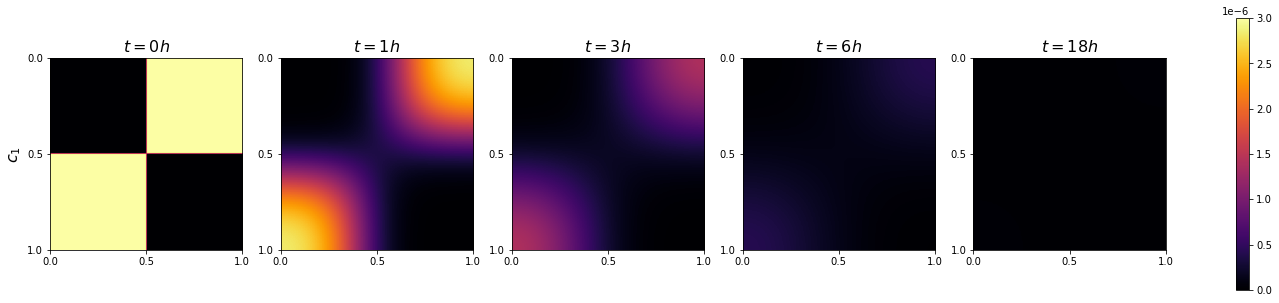
\includegraphics[width=0.75\textwidth]{../paper/assets/example-0.png} \\ 
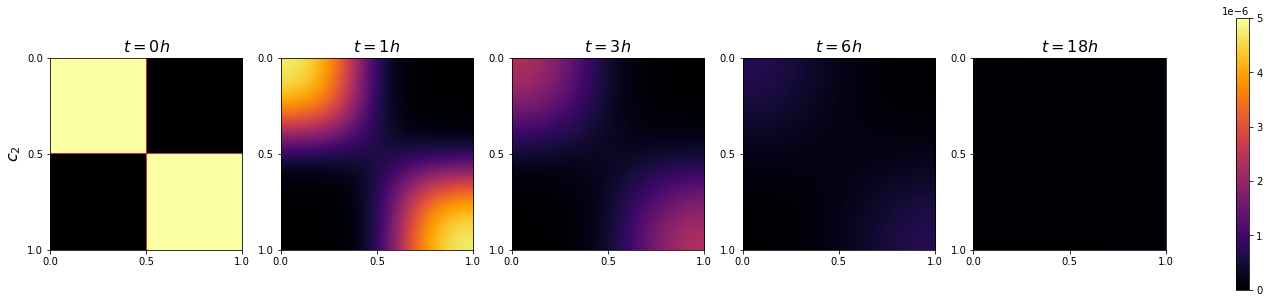
\includegraphics[width=0.75\textwidth]{../paper/assets/example-1.png} \\
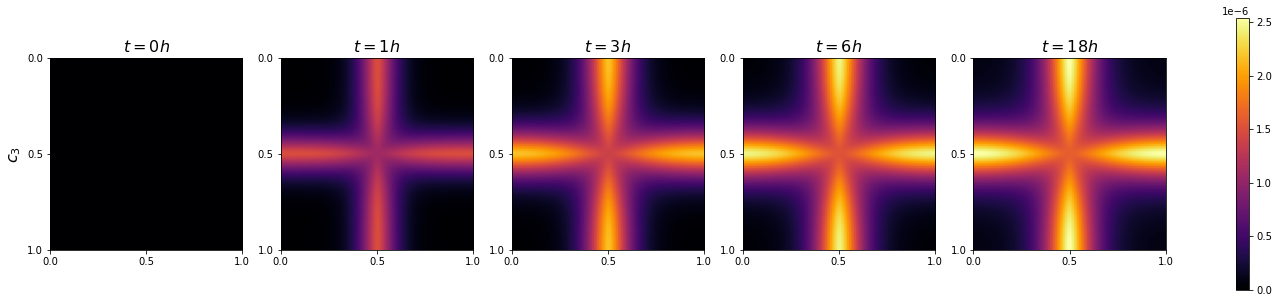
\includegraphics[width=0.75\textwidth]{../paper/assets/example-2.png}

\caption{Kompiuterinio modelio rezultato pavyzdys su parametrais gautais eksperimentiniu būdu, kai reakcija vyksta temperatūroje $T=1600\degree$ \cite{mackeviciusCloserLookComputer2012}. Parametrų reikšmės: $D = 28\times 10^{-6} \frac{\mu m^2}{s}$, $W = \sqrt[3]{10}\mu m$, $H = \sqrt[3]{10}\mu m$, $\Delta x = \frac{\sqrt[3]{10}}{79}\mu m$, $\Delta y = \frac{\sqrt[3]{10}}{79} \mu m$, $k = 192 \frac{1}{ \frac{g}{\mu m^3}\cdot s}$, $c_0 = 10^{-6} \frac{g}{\mu m^3}$, $\Delta t \approx 6.5157s$ - pasirinktas pagal \eqref{numerical-stability-condition} }

\label{result-example}
\end{figure}

\ref{result-example}-ame pavyzdys vaizduoja kompiuterinio \acs{yag} reakcijos modelio rezultatus, kurie yra išdėstyti vertikaliai kiekvienai medžiagai $c_1, c_2, c_3$. Kiekvienas kadrų stulpelis vaizduoja visų medžiagų koncentracijas tuo pačiu laiko momentu. Pavyzdyje nurodyti parametrai bus naudojami tolesniems pavyzdžiams ir nebus išreikštinai dar kartą nurodomi nebent jie keičiasi.

\subsection{Programos korektiškumo tikrinimas}

\subsubsection*{Korektiškumo tikrinimas bendru atveju}

Nagrinėjant programos korektiškumą naudosime modelio rezultatų duomenis. 
Norint nustatyti, ar programa veikia korektiškai galima tikrinti, ar mažinant žingsnių dydį, skaitinis sprendinys artėja prie tikrojo sprendinio. Šiuo atveju mažinsime erdvės žingsnius $\Delta x$ ir $\Delta y$. Tai lemia diskretaus tinklelio taškų kiekio padidėjimą, nes egzistuoja atvirkštinė priklausomybė tarp erdvinių žingsnių dydžio ir diskrečių taškų kiekio atitinkamomis ašimis (\ref{meshx}, \ref{meshy}).

\newpage

\begin{figure}[h!]
    \centering
    \caption{Kompiuterinio modelio rezultatai - sprendinio tikslumo priklausomybė nuo diskrečių taškų skaičiaus. }
    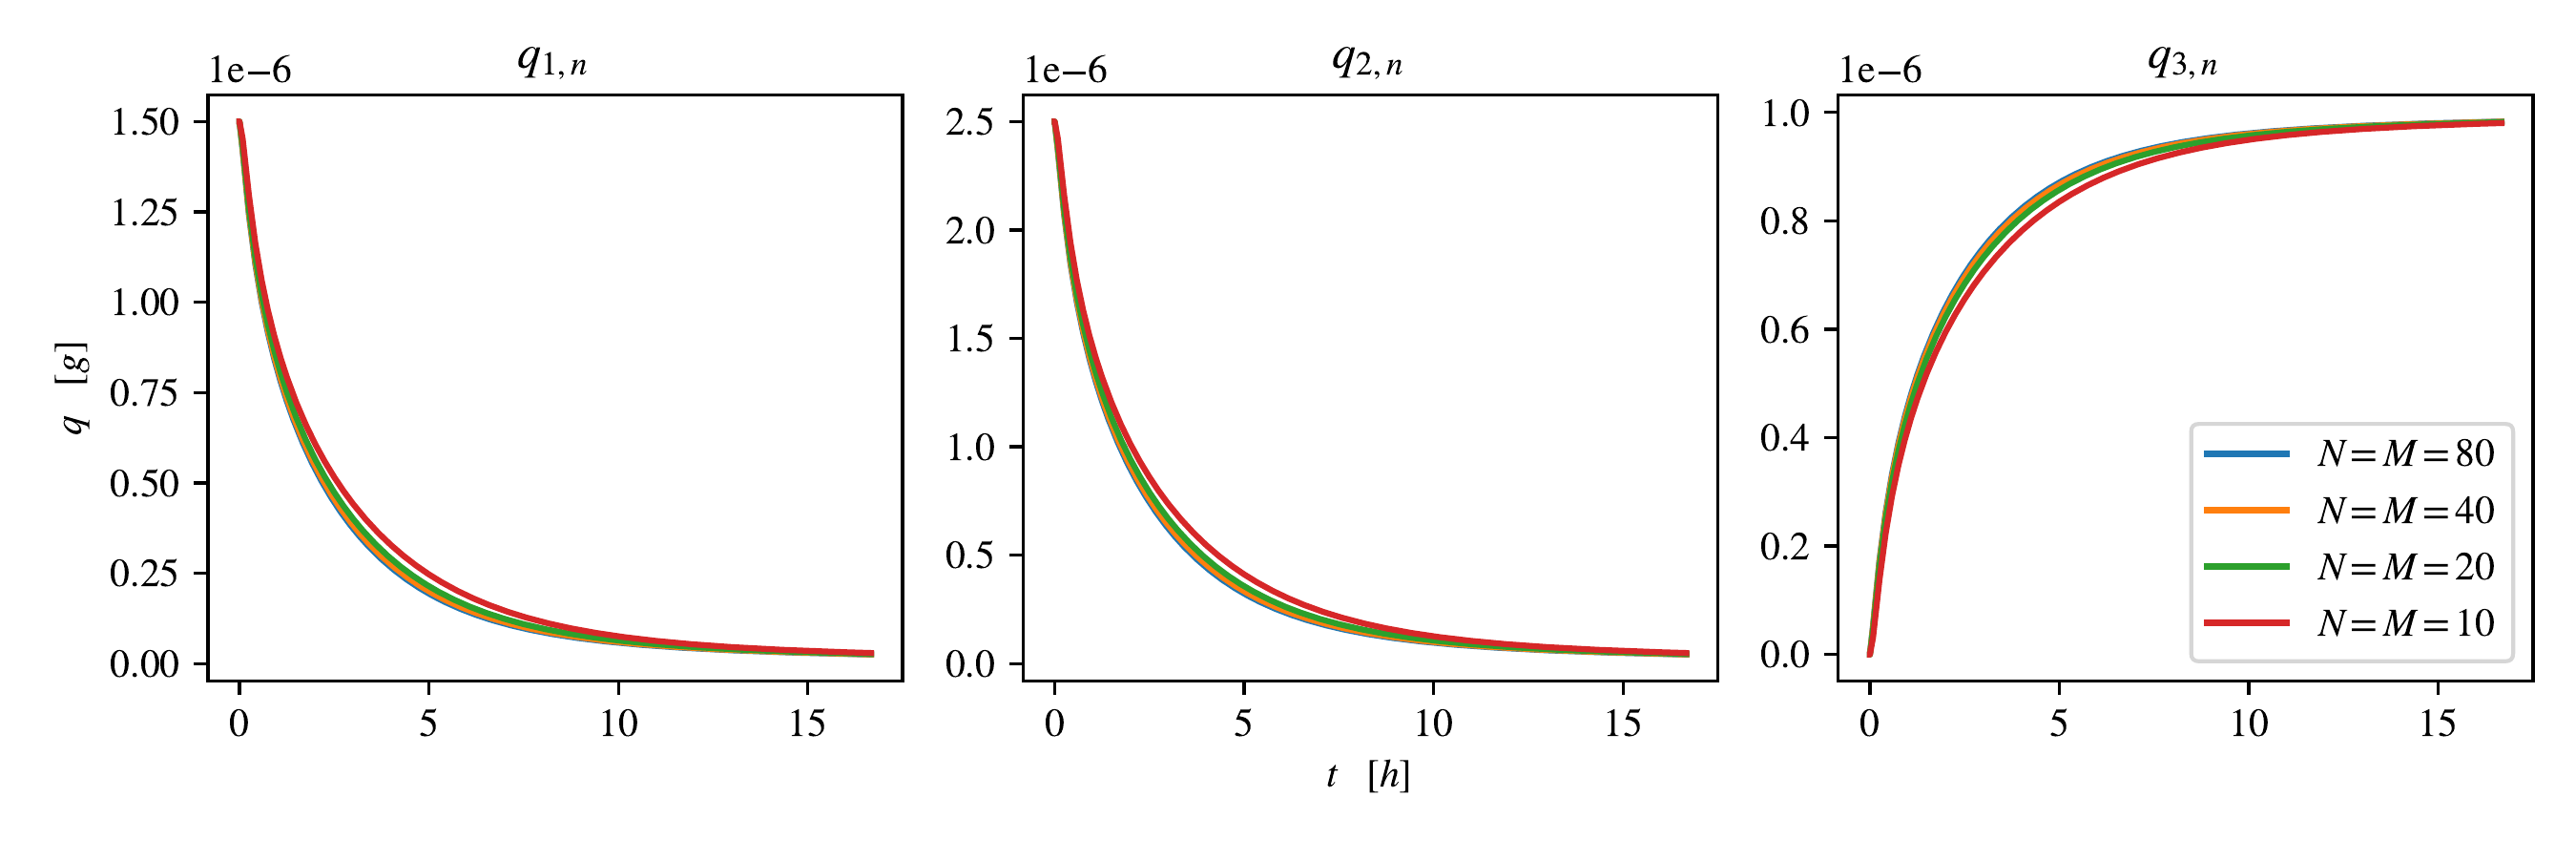
\includegraphics[width=\textwidth]{../assets/space-error-v3.png} \\
    \label{results-space-error}
\end{figure}

\ref{results-space-error}-ame pav. matome, kad eksponentiškai didinant diskrečių taškų skaičių, sprendinių grafikai tolygiai artėja prie sprendinio su didžiausiu tikslumu, darome prielaidą, kad didinant diskrečių taškų skaičių, skaitinis sprendinys konverguoją į tikrąjį sprendinį. Kažkuriuo momentu diskrečios erdvės taškų kiekio didinimas nebeduoda ypatingai didelių rezultato pagerėjimų. Sprendinių grafikuose taip pat galima įžvelgti, kad pirmų dviejų medžiagų kiekiai per laiką griežtai ne mažėja - tai mes teoriškai parodėme \eqref{negative-quantity}, taip, žinoma, yra dėl  medžiagų reakcijos. 

Analogiškai galima būtų fiksuoti erdvinius žingsnius $\Delta x, \Delta y$ ir stebėti kaip keičiasi skaitinis sprendinys mažinant laiko žingsnį $\Delta t$. Dėl priežasčių, kurios vėliau bus akivaizdžios vaizduosime du sprendinius - vienas iš jų gautas pasirinkus $\Delta t$ pagal \eqref{numerical-stability-condition}, o kitam paimta konkreti reikšmė $\Delta t = 10^{-4}$.


\begin{figure}[h!]

\centering

\caption{Kompiuterinio modelio rezultatai - sprendinio priklausomybė nuo laiko žingsio pasirinkimo. Čia reakcijos laikas $T=16h$}.

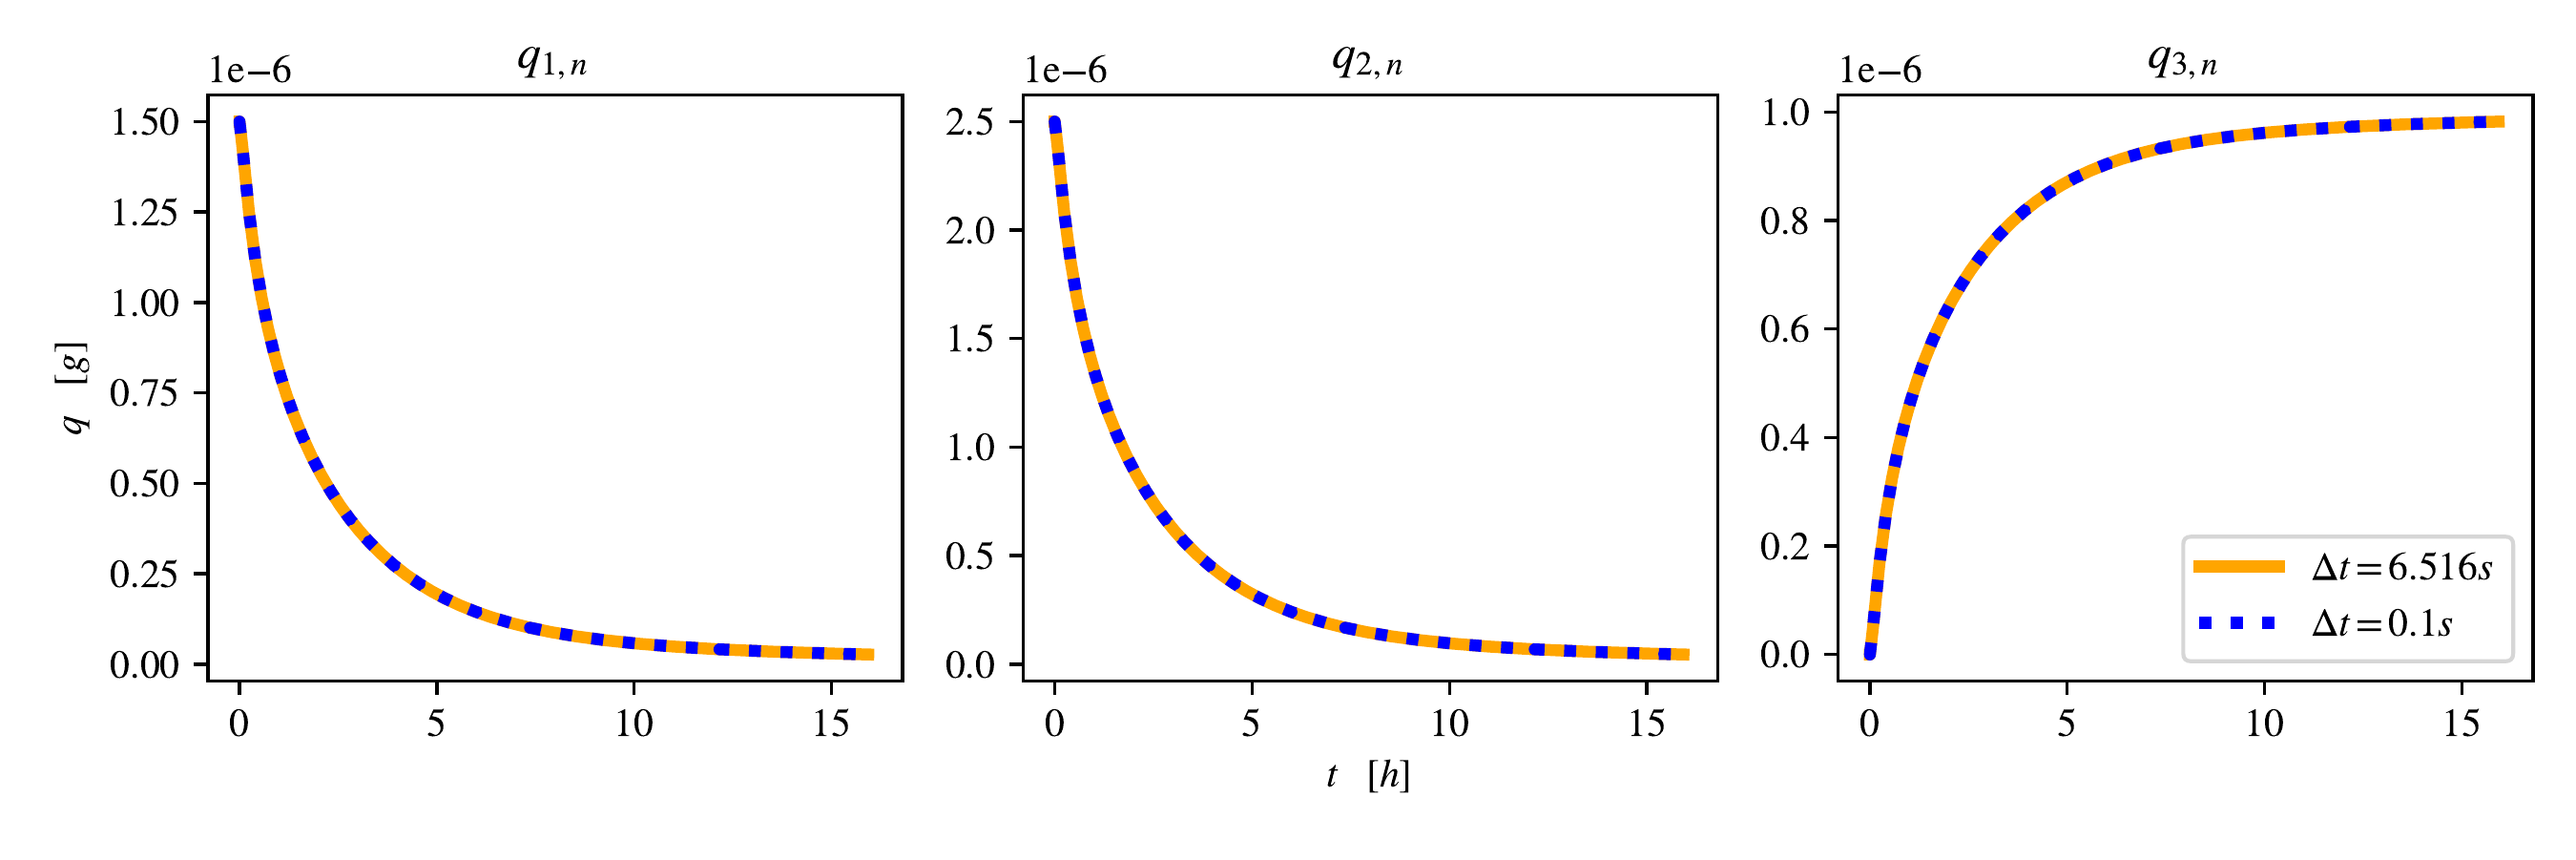
\includegraphics[width=\textwidth]{../assets/time-error-3.png}


\label{time-error}

\end{figure}

\ref{time-error}-ame pav. matome, kad sprendiniai yra identiški. Laiko žingsnio  $\Delta t$ pasirinkimas pagal \eqref{numerical-stability-condition} yra pakankamai geras ir mažesnių laiko žingsnių pasirinkimas neduoda pastebimai tikslesnių rezultatų.

\newpage
\subsubsection*{Korektiškumo tikrinimas kai vyksta tik difuzija}

Jei reakcijos koeficientas būtų lygus nuliui, vienintelis sistemoje vykstantis procesas būtų pirmų dviejų medžiagų difuzija. Jei skaitinis modelis veikia korektiškai, rezultatuose turėtų būti galima matyti, kad difuzijos metu medžiagos kiekis sistemoje nekinta, tai teoriškai parodėme skyriuje apie skaitinį stabilumą \eqref{no-q-change}.

\begin{figure}[h!]
    \centering
    \caption{Kompiuterinio modelio rezultatai - medžiagų kiekių priklausomybė nuo laiko, kai reakcija nevyksta. Čia diskrečių laiko žingsnių skaičius $\tau=10^4$, o reakcijos greitis $k = 0$. }
    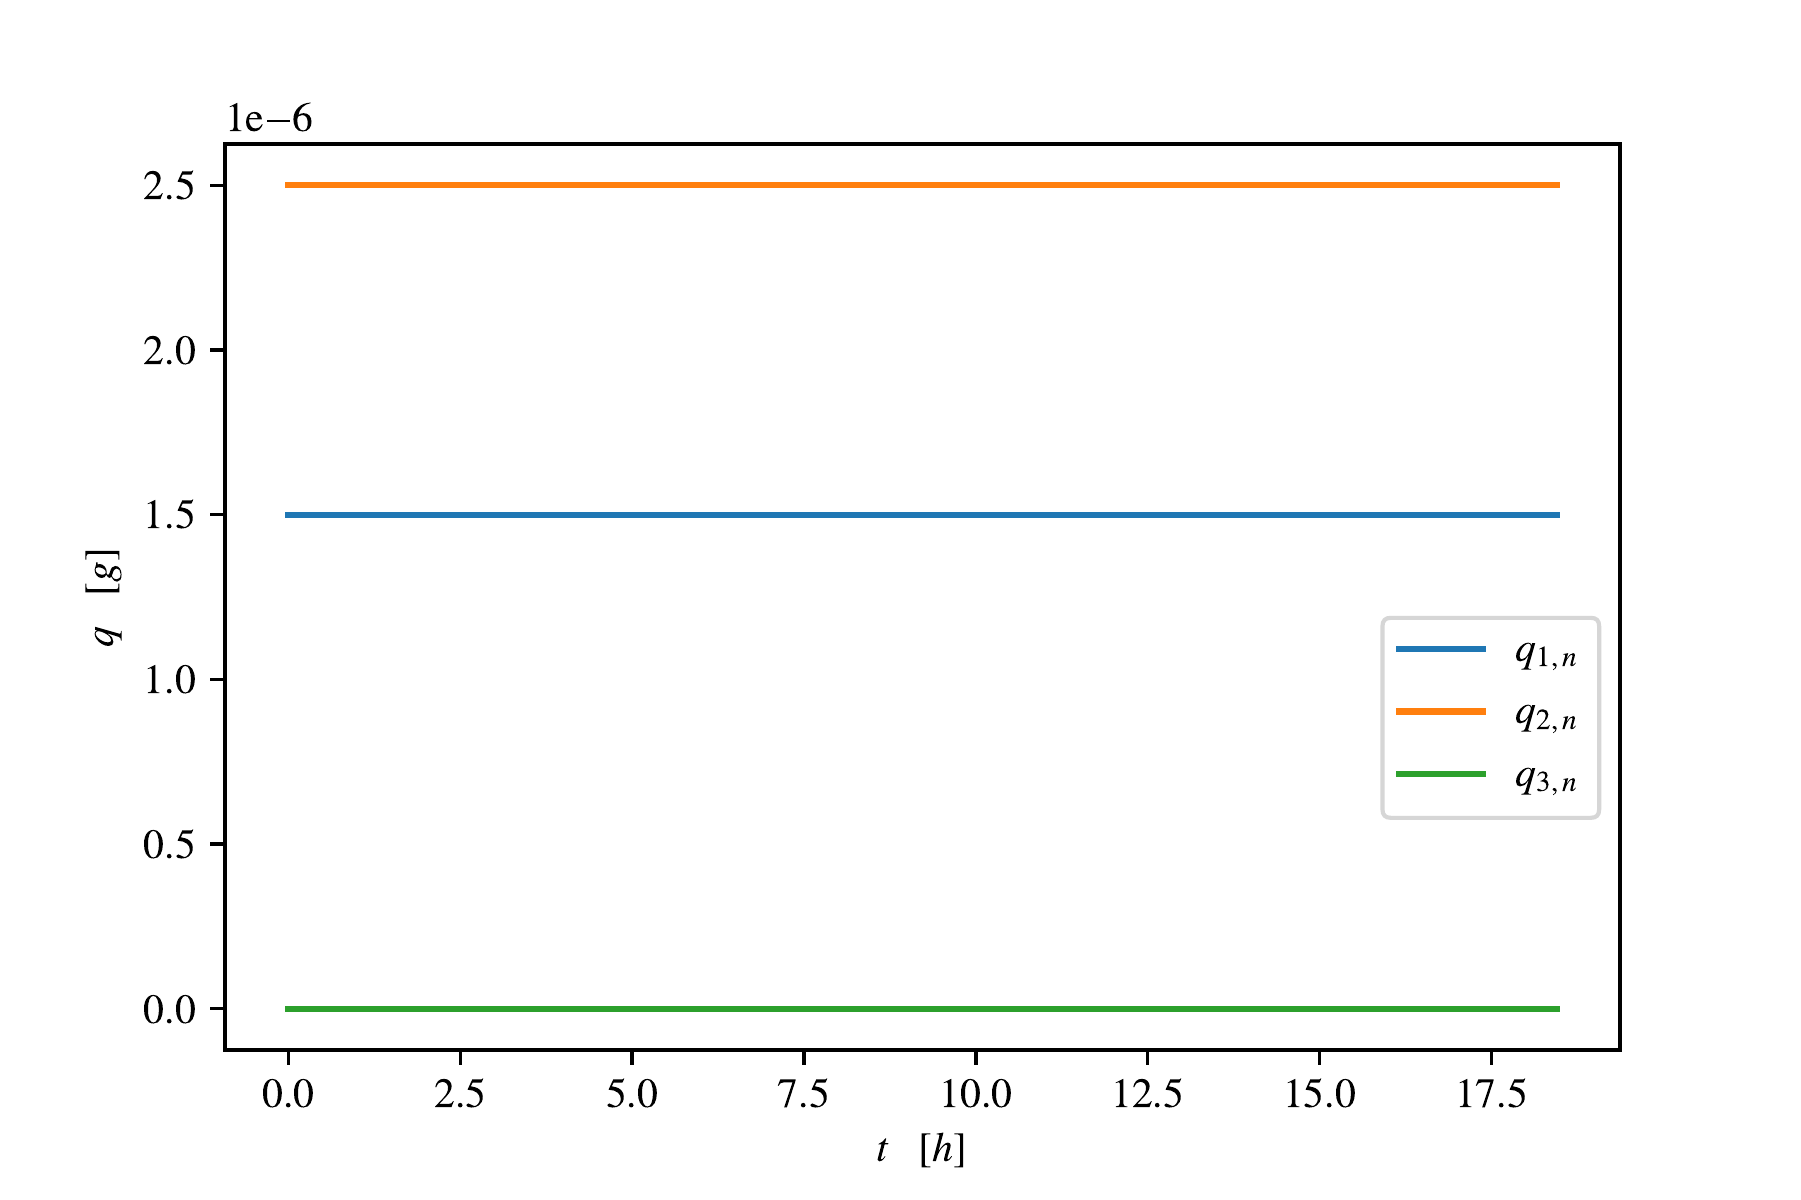
\includegraphics[width=0.5\textwidth]{../assets/only-diff-1.png}
    \label{no-reaction}
\end{figure}

\ref{no-reaction}-ame pavyzdyje kompiuterinės programos rezultatai yra būtent tokie, kokių tikėjomės, tačiau iš šio grafiko negalime užtikrinti, kad simuliacijoje išvis kažkas vyksta. Norint patikrinti, ar medžiagos difunduoja korektiškai galime pabandyti pavaizduoti medžiagų kiekį visoje srityje $\Omega$ kaip rezultatų pavyzdyje \eqref{result-example}.

\begin{figure}[h!]
\centering
\caption{Kompiuterinio modelio rezultatai - medžiagų koncentracijų pasiskirstymas per laiką, kai vyksta tik difuzija. Čia diskrečių laiko žingsnių skaičius $\tau=10^4$, o reakcijos greitis $k = 0$. }
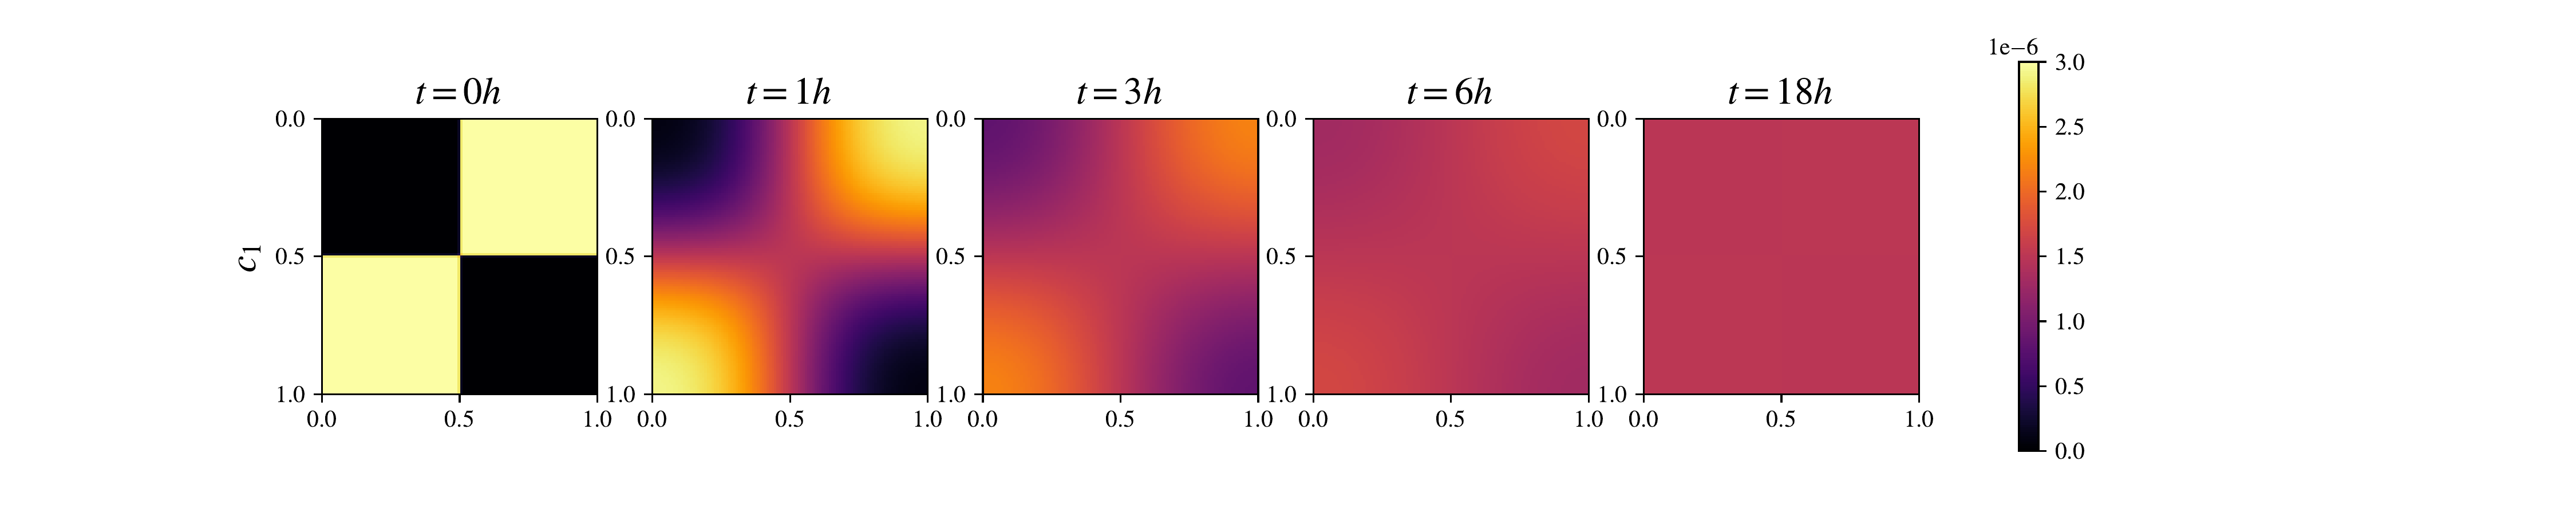
\includegraphics[width=\textwidth]{../assets/all-only-diff-1.png} \\
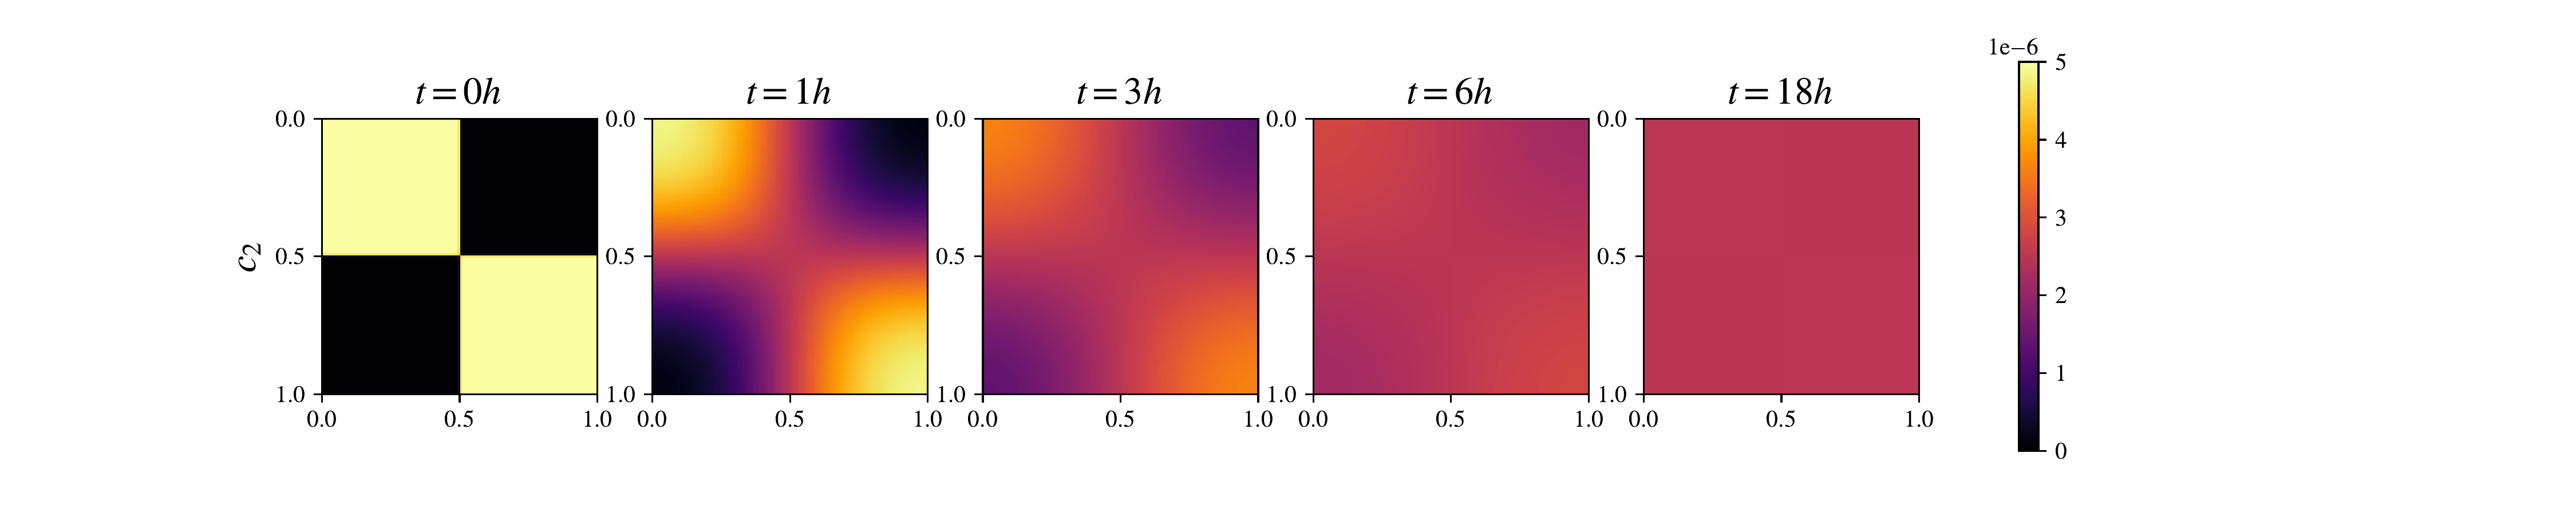
\includegraphics[width=\textwidth]{../assets/all-only-diff-2.png}
\label{only-diffusion}
\end{figure}

\ref{only-diffusion}-ame pavyzdyje akivaizdžiai matosi, kad medžiagų difuzija vyksta įprastai. Einant laikui, medžiagos iš didesnės koncentracijos sričių juda į sritis, kur koncentracija yra mažesnė. Reakcijai einant į pabaigą matome, kad medžiagos tolygiai pasiskirsto po erdvę.


